\documentclass[11pt,twoside]{scrartcl}
%\documentclass[11pt,twoside]{article}

%opening
\newcommand{\lecid}{15-316}
\newcommand{\leccourse}{Software Foundations of Security and Privacy}
\newcommand{\lecdate}{} %e.g. {October 21, 2013}
\newcommand{\lecnum}{23}
\newcommand{\lectitle}{Bootstrapping Trust}
\newcommand{\lecturer}{Matt Fredrikson}
\newcommand{\lecurl}{https://15316-cmu.github.io/index}

\usepackage{varwidth}
\usepackage{lecnotes}
\usepackage[irlabel]{bugcatch}

\usepackage{tikz}
\usetikzlibrary{automata,shapes,positioning,matrix,shapes.callouts,decorations.text,patterns,decorations.pathreplacing,matrix,arrows,chains,calc,tikzmark,petri,topaths}
\pgfdeclarelayer{bg}    % declare background layer
\pgfsetlayers{bg,main}
\usepackage{tkz-berge}
\usepackage[position=bottom]{subfig}

% \usepackage[bracketinterpret,seqinfers,sidenotecalculus]{logic}
% \newcommand{\I}{\interpretation[const=I]}

% \newcommand{\bebecomes}{\mathrel{::=}}
% \newcommand{\alternative}{~|~}
% \newcommand{\asfml}{F}
% \newcommand{\bsfml}{G}
% \newcommand{\cusfml}{C}
% \def\sqsubseteqftrule{L}%
% \def\rightrule{R}%

\begin{document}

\newcommand{\atrace}{\omega}%
%% the standard interpretation naming conventions
\newcommand{\stdI}{\dTLint[state=\omega]}%
\newcommand{\Ip}{\dTLint[trace=\atrace]}%
\newcommand{\ws}{\omega}\newcommand{\wt}{\nu}% 

\newcommand{\aff}[2]{\ensuremath{#1~\keywordfont{aff}~#2}}
\newcommand{\ownsr}{\ensuremath{\keywordfont{owns}}}
\newcommand{\isfac}{\ensuremath{\keywordfont{isFaculty}}}
\newcommand{\studof}{\ensuremath{\keywordfont{studentOf}}}
\newcommand{\canopen}{\ensuremath{\keywordfont{canOpen}}}
\newcommand{\matt}{\ensuremath{\mathsf{mfredrik}}\xspace}
\newcommand{\tli}{\ensuremath{\mathsf{bob}}\xspace}
\newcommand{\admin}{\ensuremath{\mathsf{admin}}\xspace}
\newcommand{\jan}{\ensuremath{\mathsf{janh}}\xspace}
\newcommand{\frank}{\ensuremath{\mathsf{fp}}\xspace}
\newcommand{\office}{\ensuremath{\mathsf{cic2126}}\xspace}
\newcommand{\eduroam}{\ensuremath{\mathsf{er}}\xspace}
\newcommand{\cmu}{\ensuremath{\mathsf{cmu}}\xspace}
\newcommand{\ca}{\ensuremath{\mathsf{CA}}\xspace}
\newcommand{\tca}{\ensuremath{\mathsf{TrustedCA}}\xspace}
\newcommand{\dca}{\ensuremath{\mathsf{DiscountCA}}\xspace}
\newcommand{\isstu}{\ensuremath{\keywordfont{isStudent}}\xspace}
\newcommand{\canacc}{\ensuremath{\keywordfont{canAccess}}\xspace}

\newcommand{\pk}[1]{\ensuremath{\keywordfont{pk}_{#1}}\xspace}
\newcommand{\sk}[1]{\ensuremath{\keywordfont{sk}_{#1}}\xspace}
\newcommand{\isca}[1]{\ensuremath{\keywordfont{isCA}(#1)}\xspace}
\newcommand{\cert}[2]{\ensuremath{\keywordfont{cert}_{#1 \to #2}}\xspace}
\newcommand{\iskey}[2]{\ensuremath{\keywordfont{isKey}(#1,#2)}\xspace}
\newcommand{\sign}[2]{\ensuremath{\keywordfont{sign}_{#1}(#2)}\xspace}
\newcommand{\verify}[2]{\ensuremath{\keywordfont{verify}_{#1}(#2)}\xspace}
\newcommand{\encr}[2]{\ensuremath{\keywordfont{enc}_{#1}(#2)}\xspace}
\newcommand{\trusts}[1]{\ensuremath{\keywordfont{trusts}(#1)}\xspace}

\newdimen{\linferenceRulehskipamount}
\linferenceRulehskipamount=2em
  \linferenceRulevskipamount=0.6em

% \newcommand{\lowt}{\lowsec}
% \newcommand{\hight}{\hisec}

\lstdefinestyle{customc}{
  belowcaptionskip=1\baselineskip,
  breaklines=true,
  language=C,
  showstringspaces=false,
  numbers=none,
  % xleftmargin=1ex,
  framexleftmargin=1ex,
  % numbersep=5pt,
  % numberstyle=\tiny\color{mygray},
  basicstyle=\footnotesize\ttfamily,
  keywordstyle=\color{blue},
  commentstyle=\itshape\color{purple!40!black},  
  stringstyle=\color{orange},
  morekeywords={output,assume,observe,input,bool,then,fun,match,in,val,list,type,of,string,unit,let,bytes,mov,imul,add,sar,shr,function,forall,nat,requires,ensures,method,returns,assert,new,array,modifies,reads,old,predicate,lemma,seq,calc,nan,var,exists,invariant,decreases,datatype,declassify,uint8},
  tabsize=2,
  deletestring=[b]',
  backgroundcolor=\color{gray!15},
  frame=tb
}
\lstset{escapechar=@,style=customc}

\maketitle
\thispagestyle{empty}

%%%%%%%%%%%%%%%%%%%%%%%%%%%%%%%%%%%%%%%%%%%%%%

\section{Introduction}

When we discussed authorization logic, we briefly touched on the topic of trust. More specifically, authorization logic is distinguished from other logics that we have looked at by the $\says{A}{\ausfml}$ construct that represents the fact that principal $A$ states proposition $\ausfml$. We saw how to encode \emph{decentralized} security policies for systems using \keywordfont{says}, so that various entities can define their own access control rules. The system components that must ultimately either grant or deny access to resources can decide which principals to trust, and subsequently implement a policy by only accepting \keywordfont{says} proclamations from trusted principals.

We illustrated this using the Grey system~\cite{Bauer2005}, and now we will see a different example that emphasizes the importance of organized trust when making policy decisions. You may be familiar with the eduroam service, which provides members of participating academic institutions with wireless network access when they visit another institution. For example, because both CMU and Pitt are members of eduroam, when you visit the Pitt campus you can join the wireless SSID \verb'eduroam', and provide your Andrew ID and password to use the internet. The same is true at thousands of other institutions across the world that subscribe to this service.

If you stop to think about it, this is somewhat remarkable given the scale and disparity in geography and governance among the institutions. How does Pitt know that you have entered the valid credentials for your Andrew account, which is managed by CMU? A naive solution might be to distribute the credentials of \emph{all} users at eduroam institutions to all of the institutions. Obviously this won't scale, so perhaps a decentralized authorization policy is called for. First of all, the service \eduroam can delegate the responsibility of deciding who is currently a student to the various institutions, for example as shown in Equation~\ref{eq:edu1}. We use \eduroam to denote the eduroam principal.
\begin{equation}
\label{eq:edu1}
P_1 \equiv \says{\eduroam}{(\forall x.(\says{\cmu}{\isstu(x)}) \limply \isstu(x))}
\end{equation}
Then the main policy governing access to the eduroam wireless network is shown in Equation~\ref{eq:edu2}
\begin{equation}
\label{eq:edu2}
P_2 \equiv \says{\eduroam}{(\forall x.\isstu(x) \limply \canacc(x))}
\end{equation}
The wireless access points responsible for providing the service can use (\ref{eq:edu1}) and (\ref{eq:edu2}) as assumptions $\Gamma$ to construct or check a proof of the judgement in Eq~\ref{eq:edu3} when student $x$ attempts to use the service.
\begin{equation}
\label{eq:edu3}
\lsequent{\Gamma}{\says{\eduroam}{\canacc(x)}}
\end{equation}
For example, suppose that Bob attempts to do so. Let us use the following symbols.
\begin{align*}
P_3 &\equiv \forall x.(\says{\cmu}{\isstu(x)}) \limply \isstu(x) \\
P_4 &\equiv \forall x.\isstu(x) \limply \canacc(x) \\
P_5 &\equiv \isstu(x) \limply \canacc(x)
\end{align*}
Then the proof begins as follows.
\begin{sequentdeduction}[array]
\linfer[saysr]{
  \linfer[saysl+saysl] {
    \linfer[alll] {
      \linfer[implyl] {
        \vdots
        !\linfer[aff+id] {
          \lclose
        } {
          \lsequent{P_3,\canacc(\tli)}{\aff{\eduroam}{\canacc(\tli)}}
        }
      } {
        \lsequent{P_3,P_5}{\aff{\eduroam}{\canacc(\tli)}}
      }
    } {
      \lsequent{P_3,P_4}{\aff{\eduroam}{\canacc(\tli)}}
    }
  } {
    \lsequent{\Gamma}{\aff{\eduroam}{\canacc(\tli)}}
  }
}{
  \lsequent{\Gamma}{\says{\eduroam}{\canacc(\tli)}}
}
\end{sequentdeduction}
The elided left branch of the proof after \irref{implyl} proves that \tli is a student from $P_3$.
\begin{sequentdeduction}
\linfer[alll] {
  \linfer[implyl] {
    \lsequent{}{\says{\cmu}{\isstu(\tli)}}
    &\linfer[id]{\lclose}{\lsequent{\isstu(\tli)}{\isstu(\tli)}}
  } {
    \lsequent{(\says{\cmu}{\isstu(\tli)}) \limply \isstu(\tli)}{\isstu(\tli)}
  }
} {
  \lsequent{\forall x.(\says{\cmu}{\isstu(x)}) \limply \isstu(x)}{\isstu(\tli)}
}
\end{sequentdeduction}
In order to complete this proof, the access point needs to be able to assume that \cmu states that \tli is currently a student. In fact, because the derivation above will be about the same for any user, except for the details of institution and user names, the endpoint need not recompute or check it for each login. Access boils down to a trusted institution's endorsement that the user is legitimate and eligible for the service, so instead perhaps users' devices can just send evidence of the endorsement directly, or the endpoint can obtain it by some other means.

But how can the access point be sure that this evidence is authentic? We hinted in the last lecture that digital signatures utilizing cryptography are a common solution. But the cryptographic techniques that enable digital signatures require \emph{keys}, which are either secrets distributed among trustworthy parties, or public objects that can be reliably associated with individuals or organizations.

For example, \cmu could sign and date a certificate stating that \tli is currently a student, perhaps with a timeout to account for Bob's expected graduation date. It would do so using its \emph{private key}, known only to CMU, and the access point would verify it by checking the signature against \cmu's \emph{public key}. How does the access point know that it is using the correct public key? What if someone tricked it into using a different public key, associated with an attacker's private key, so that it would trust statements signed by the attacker as coming from \cmu? 

We will address this topic today, looking more closely at digital certificates and \emph{Public Key Infrastructure} (PKI), which is a distributed mechanism for managing the trust needed to solve the problems introduced in this example.

\section{Digital Certificates \& Certificate Authorities}

For the rest of this lecture, we will assume that all principals $A$ have a secret key \sk{A} and a public key \pk{A}. Suppose in the context of the running example from the previous section that the \eduroam principal generates the public, private key pairs for all participating institutions. 

\paragraph{Digital signatures.} One of the main applications of public/secret key pairs is to \emph{digital signatures}, which we have referenced informally before. A digital signature scheme consists of three algorithms, for generating keys, signing messages, and verifying signatures, respectively. We will always assume that public/secret key pairs have been generated correctly by some existing means, so we won't spend any time discussing the key generation algorithm. It is useful however to look a bit more closely at the latter two algorithms, $\sign{\sk{A}}{m}$ and $\verify{\pk{A}}{s}$, to understand how signatures are used to establish trust.

The signing algorithm $\sign{\sk{A}}{m}$ takes as input a secret key \sk{A} for a principal $A$ in addition to a message $m$, and outputs a signature $s$. The verification algorithm $\verify{\pk{A}}{s}$ takes as input a public key $\pk{A}$ for a principal $A$ and a signature $s$, and outputs either $\strue$ or $\sfalse$. \emph{If and only if} the signature was produced by calling $\keywordfont{sign}$ with $A$'s secret key \sk{A}, i.e. $s = \sign{\sk{A}}{m}$ for some $m$, then $\verify{\pk{A}}{s} = \strue$. Otherwise, $\verify{\pk{A}}{s} = \sfalse$. So in particular $\verify{\pk{A}}{s}$ will return false if $s$ is a signature created with the secret key of some other principal $B \ne A$, or more formally $\verify{\pk{A}}{\sign{\sk{B}}{m}} = \sfalse$ for all $m$. This is summarized in (\ref{eq:digsig}).
\begin{equation}
\label{eq:digsig}
\verify{\pk{A}}{s} =
\left\{
\begin{array}{ll}
\strue & \text{if}~s = \sign{\sk{A}}{m}~\text{for some}~m \\
\sfalse & \text{otherwise}
\end{array}
\right.
\end{equation}
Technically speaking, the behavior specified in (\ref{eq:digsig}) is only required to hold with overwhelming probability over the keys produced by the generator~\cite{Katz2014}. For our purposes however, it is fine to think of (\ref{eq:digsig}) as holding all the time.

The essential property established by (\ref{eq:digsig}) is \emph{unforgeability}. As long as \sk{A} remains a secret, and the only individual who knows the value of \sk{A} is $A$, then the only messages that $\verify{\pk{A}}{\cdot}$ will return \strue on are those that $A$ actually signed with \sk{A}. Of course, if one wanted to forge a message with $A$'s signature, they could attempt to guess $\sk{A}$, which is why it is important that secret keys be chosen completely randomly from a very large space of possibilities. It is also important that the outputs of $\sign{\sk{A}}{\cdot}$ reveal no information about $\sk{A}$ that can help one guess the secret key with greater probability. We will assume that all of these facts hold for the secret keys and digital signatures used for the rest of the lecture, and we will also assume that if \sk{A} was generated by someone other than $A$ (e.g., \eduroam in our running example), then they are trusted not to sign messages on $A$'s behalf.

\paragraph{Certificates.}
Because \eduroam knows for a fact that CMU's public key \pk{\cmu} is associated with the correct principal, it can generate a \emph{certificate} that asserts this fact with its signature.
\begin{equation}
\label{eq:cert}
\cert{\eduroam}{\cmu} \equiv \sign{\sk{\eduroam}}{\iskey{\cmu}{\pk{\cmu}}}
\end{equation}
In (\ref{eq:cert}), the predicate $\iskey{\cmu}{\pk{\cmu}}$ denotes the fact that the public key $\pk{\cmu}$ belongs to, or is uniquely associated with, the principal \cmu. \eduroam signs with its secret key \sk{\eduroam} to authenticate the certificate, as no other principals should have knowledge of \sk{\eduroam} and so only \eduroam itself could have produced the cert.

Now if \cmu wants to convince one of the access points that Bob is in fact a student, it can use \cert{\eduroam}{\cmu} as part of a sequence of messages to do so as shown in (\ref{eq:certmsg}).
\begin{equation}
\label{eq:certmsg}
\pk{\cmu}, \cert{\eduroam}{\cmu}, \sign{\sk{\cmu}}{\isstu(\tli)}
\end{equation}
As long as the access point has \eduroam's public key \pk{\eduroam}, then it will be able to verify that \cert{\eduroam}{\cmu} is indeed signed by \eduroam, and so \pk{\cmu} must really belong to \cmu, and then use \pk{\cmu} to verify that \cmu signed $\isstu(\tli)$. \cmu can send this information to the access point over an insecure channel, and the access point will still be able to trust the final conclusion.

\paragraph{Certificate authorities.}
Certificates enable the extension of trust to new principals from pre-existing trust relationships. In our running example, \eduroam is trusted by all access points to issue certificates for the public keys of other principals. In general, parties endowed with this sort of trust are called \emph{certificate authorities} (CAs). The job of a CA is to issue digital certificates that associate principals with public keys, so in our example the CA is \eduroam.

The CA uses their own public/secret key pair to issue certificates, so those who wish to verify certificates issued by a particular CA need a reliable and secure way of obtaining the CA's public key. We will discuss several alternatives for achieving this in the next section, but for now it is fine to assume that all principals are in posession of the correct public key for the CA.

\subsection{Formalizing certificates and trust}

Now that we have seen how signatures and certificates are used to extend trust relationships, let's think about how to incorporate this into our reasoning about authorization. Specifically, we will formalize policies that utilize signatures, certificates, and trust in the CA so that these elements can be used with existing policies written in authorization logic. We will encapsulate this in a set of policies that can supplement the assumptions used in a proof, but one could alternatively incorporate these principles into axioms in the logic and devise corresponding proof rules~\cite{bauer:thesis}.

The first way in which we might want to use signatures is to introduce \verb'says' terms. Namely, if we are in posession of a proposition $P$ signed with \sk{A}, and we know that \sk{A} is the secret key of $A$, then we can conclude that $\says{A}{\ausfml}$. We will denote this policy $C_1$ as formalized in Equation~\ref{eq:signaxiom}.
\begin{equation}
\label{eq:signaxiom}
C_1 \equiv \forall x . \iskey{x}{\pk{x}} \limply \sign{\sk{x}}{\ausfml} \limply \says{x}{\ausfml}
\end{equation}
The assumption that makes $C_1$ reasonable is that if a principal is willing to sign something, then they are prepared to state it as well. In the base authorization logic, if our proof goal is a \verb'says' term, then we had no choice but to apply \irref{saysr} and subsequently prove an affirmation judgement. It is not difficult to see that $C_1$ gives us an alternative way of proving such goals, namely that whenever $C_1$ is in our assumptions then we can prove $\says{A}{\ausfml}$ by proving $\sign{\sk{A}}{\ausfml}$ and $\iskey{A}{\pk{A}}$ from the other assumptions.

\begin{lemma}
\label{lemma:sign}
The \irref{sign} rule is applicable whenever $C_1$ is used as a policy.
\[
\cinferenceRule[sign|Sign]{sign}
{\linferenceRule[sequent]
  {
    \lsequent{\Gamma,C_1}{\iskey{A}{\pk{A}}}
    &\lsequent{\Gamma,C_1}{\sign{\sk{A}}{\ausfml}}
  }
  {\lsequent{\Gamma,C_1}{\says{A}{\ausfml}}}
}{}%
\]
\end{lemma}
\begin{proof}
This proof is a straightforward sequent deduction that does not use any rules specific to authorization logic.
\begin{sequentdeduction}
\linfer[alll] {
  \linfer[implyl] {
    \lsequent{\Gamma}{\iskey{A}{\pk{A}}}
    \ &\linfer[implyl] {
      \lsequent{\Gamma}{\sign{\sk{A}}{\ausfml}}
      \ &\linfer[id]{\lclose}{\lsequent{\Gamma,\says{A}{\ausfml}}{\says{A}{\ausfml}}}
    } {
      \lsequent{\Gamma,\sign{\sk{A}}{\ausfml} \limply \says{A}{\ausfml}}{\says{A}{\ausfml}}
    }
  } {
    \lsequent{\Gamma,\iskey{A}{\pk{A}} \limply \sign{\sk{A}}{\ausfml} \limply \says{A}{\ausfml}}{\says{A}{\ausfml}}
  }
} {
  \lsequent{\Gamma,\forall x . \iskey{x}{\pk{x}} \limply \sign{\sk{x}}{\ausfml} \limply \says{x}{\ausfml}}{\says{A}{\ausfml}}
}
\end{sequentdeduction}
\end{proof}

Now that we have a way of converting signatures into statements, we want to apply this towards formalizing the trust extension principle behind certificate authorities and the certificates that they issue. Recall that the trust placed in CAs is that they will sign messages that reliably tell us which principals are bound to particular public keys. So if we know that $A$ is a certificate authority, and we have a certificate $\cert{A}{B}$, then this principle lets us conclude that $\pk{B}$ belongs to $B$. We formalize this as shown in Eq.~\ref{eq:certlongaxiom}.
\begin{equation}
\label{eq:certlongaxiom}
\forall x.\forall y. \isca{x} \limply \cert{x}{y} \limply \iskey{y}{\pk{y}}
\end{equation}
However, $\cert{x}{y}$ is just a shorthand for $\sign{\sk{x}}{\iskey{y}{\pk{y}}}$. Using the \irref{sign} rule above we can always convert $\cert{x}{y}$ into $\says{x}{\iskey{y}{\pk{y}}}$. Moreover, we might imagine that there could arise situations where the CA $x$ never explicitly signed a message asserting the binding between $y$ and $\pk{y}$, but using other assumptions in our policy we can apply the rules of authorization logic to conclude that $x$ is willing to say $\iskey{y}{\pk{y}}$. A more general policy that embodies our trust in the CA is $C_2$ as shown in Eq.~\ref{eq:certaxiom}.
\begin{equation}
\label{eq:certaxiom}
C_2 \equiv \forall x.\forall y. \isca{x} \limply (\says{x}{\iskey{y}{\pk{y}}}) \limply \iskey{y}{\pk{y}}
\end{equation}
Just as the \irref{sign} rule simplifies the use of $C_1$ in proofs, the \irref{cert} rule does so for $C_2$.
\begin{lemma}
\label{lemma:cert}
The \irref{cert} rule is applicable whenever $C_2$ is used as a policy.
\[
\cinferenceRule[cert|Cert]{cert}
{\linferenceRule[sequent]
  {
    \lsequent{\Gamma,C_2}{\isca{A}}
    &\lsequent{\Gamma,C_2}{\says{A}{\iskey{B}{\pk{B}}}}
  }
  {\lsequent{\Gamma,C_2}{\iskey{B}{\pk{B}}}}
}{}%
\]
\end{lemma}
\begin{proof}
Just like in the proof on Lemma~\ref{lemma:sign}, this fact follows directly from propositional rules. We omit it here as it should be easy to check.
\end{proof}

\subsection{Closing out the example}

Now that we understand how certificate authorities, digital signatures, and certificates work, let's return to the example from the beginning and show how to use these elements to finish the proof. Recall that we had worked the proof to a single proof obligation, which is the judgement $\lsequent{}{\says{\cmu}{\isstu(\tli)}}$. Obviously we will not be able to prove this judgement, so instead let's consider what assumptions we might add to the system to make this goal provable.


We began the discussion in this section by observing that the access point responsible for discharging or checking this goal needs to be able to trust the \cmu actually does say that Bob is a student. We then introduced signatures and certificates, and reasoned that \cmu could send the messages in (\ref{eq:certmsg}) to the access point.
\[
\pk{\cmu}, \cert{\eduroam}{\cmu}, \sign{\sk{\cmu}}{\isstu(\tli)}
\]
This suggests that the access point should have $Q_1$ and $Q_2$ below, as \cert{\eduroam}{\cmu} is shorthand for $Q_1$ and $Q_2$ is \cmu's signed statement about Bob's status.
\begin{align}
Q_1 &\equiv \sign{\sk{\eduroam}}{\iskey{\cmu}{\pk{\cmu}}} \\
Q_2 &\equiv \sign{\sk{\cmu}}{\isstu(\tli)}
\end{align} 
Of course, to reason from these assumptions it will also need the policies $C_1,C_2$ that we just introduced, so that the simpler \irref{sign} and \irref{cert} rules can take effect. Finally, the access point will need to assume that \eduroam is a certificate authority. 
\begin{equation}
Q_3 \equiv \isca{\eduroam}
\end{equation}
This is reasonable and practical, as the access points are provisioned specifically to support the eduroam service, and so during setup we can assume that the correct public key for \eduroam is loaded into memory. So our assumptions $\Gamma = Q_1,Q_2,Q_3,C_1,C_2$.

To complete the proof, we ultimately would like to use \cmu's signed statement to obtain the objective. We apply \irref{sign}, and immediately close out one branch because of assumptoin $Q_2$.
\begin{sequentdeduction}[array]
\linfer[sign] {
  \lsequent{\Gamma} {\iskey{\cmu}{\pk{\cmu}}}
  !\linfer[id]{\lclose}{\lsequent{\Gamma} {\sign{\sk{\cmu}}{\isstu(\tli)}}}
} {
  \lsequent{\Gamma} {\says{\cmu}{\isstu(\tli)}}
}
\end{sequentdeduction}
Our remaining obligation is to prove that \pk{\cmu} is in fact \cmu's public key. We can use \irref{cert} because of $Q_3$, but we then also need to apply \irref{sign} again to get \eduroam's cert into a statement.
\begin{sequentdeduction}[array]
\linfer[sign] {
  \linfer[id]{\lclose}{\lsequent{\Gamma}{\isca{\eduroam}}}
  !\linfer[sign] {
    \linfer[id]{\lclose}{\lsequent{\Gamma}{\iskey{\eduroam}{\pk{\eduroam}}}}
    !\linfer[id]{\lclose}{\lsequent{\Gamma}{\sign{\sk{\eduroam}}{\iskey{\cmu}{\pk{\cmu}}}}}
  } {
    \lsequent{\Gamma}{\says{\eduroam}{\iskey{\cmu}{\pk{\cmu}}}}
  }
} {
  \lsequent{\Gamma} {\iskey{\cmu}{\pk{\cmu}}}
}
\end{sequentdeduction}

This completes the proof. Now the access point can conclude that \cmu vouches for Bob, and so according to the original eduroam policy ($P_1$ and $P_2$ in Eqs.~\ref{eq:edu1} and \ref{eq:edu2}) that he is allowed to use the network. But notice how the access point is able to draw this conclusion by trusting only the CA, \eduroam in the beginning, and not \cmu or \tli. From this initial seed of trust it was able to ``bootstrap'' the additional trust assumptions that it needed to apply the authorization policy. This idea of bootstrapping trust from a few entities to many through CA designations is a key takeaway of this lecture, and one that is widely used in practice to enforce authorization on large-scale distributed systems.

\subsection{Failure modes} 

Can principals always rely on certificates and trust relationships to establish authenticity of messages? There are a few situations that the access point needs to worry about, and they have to do with the assumption that \emph{private keys are only known to their respective principals}. If this assumption ever fails, then problems can crop up in a few places in our running example.

The first case where the assumption can fail is for \cmu. Supposing that \cmu's private key used for signing messages (e.g., \sign{\sk{\cmu}}{\isstu(\tli)}) becomes compromised and leaks to an untrusted individual who is not authorized to make statements on behalf of \cmu. Then this person can sign messages of their choosing and have others who believe that \pk{\cmu} belongs to \cmu believe them with reasonable evidence. In the context of the example, that individual could sign things that are patently false, such as $\isstu(\mathsf{beyonce})$, and the access point would believe that the messages originated from \cmu. Recalling that the assertion $\says{\cmu}{\isstu(x)}$ is the only thing one needs to establish to access the network, this obviously renders the access control ineffective.

The other case corresponding to compromise of \eduroam's secret key has similar consequences when considered in the context of our example. If an attacker is in possession of \eduroam's secret key, then they gain the ability to generate certificates that look like they came authentically from \eduroam. So rather than using \cmu's secret key directly, this attacker would generate a separate public/secret key pair $\pk{\star},\sk{\star}$, and use \eduroam's key to certify that \pk{\star} belongs to \cmu.
\begin{equation}
\label{eq:certbad}
\cert{\eduroam}{\cmu^\star} \equiv \sign{\sk{\eduroam}}{\iskey{\cmu}{\pk{\star}}}
\end{equation}
They could then convince the access point to allow any principal of their choosing to use the network, sending the messages shown in (\ref{eq:certmsgbad}).
\begin{equation}
\label{eq:certmsgbad}
\pk{\star}, \cert{\eduroam}{\cmu^\star}, \sign{\sk{\star}}{\isstu(\mathsf{beyonce})}
\end{equation}
As in the previous case, compromise of the secret key \sk{\eduroam} renders the access control system pointless. 

But outside the narrow context of our example, compromise of signing keys belonging to parties that are widely trusted to certify identities and establish policies is extremely serious. Without additional measures in place that we will discuss later, it gives one the ability to fabricate and steal the identities of arbitrary individuals. This can have dire consequences. 

For example, suppose that $A$ and $B$ wish to communicate using their public and private keys. They trust certificates signed by $C$, and so if $A$ wishes to send $B$ an encrypted message, then $B$ will first send $A$ their public key $\pk{B}$ and a certificate issued by $C$ that attests to the validity of that public key. Then $A$ can encrypt the message using $B$'s public key, $\encr{\pk{B}}{\ldots}$, and $B$ will be able to decrypt with their secret key $\sk{B}$.

\begin{center}
\begin{tabular}{ccc}
$A$ & & $B$ \\
\tikzmark{m3} & \pk{B},$\sign{\sk{C}}{\iskey{B}{\pk{B}}}$ & \tikzmark{m4} \\[1ex]
\tikzmark{m5} & $\encr{\pk{B}}{\text{``Hello!''}}$ & \tikzmark{m6}
\end{tabular}
\begin{tikzpicture}[overlay, remember picture, yshift=2*\baselineskip]
  \draw [thick,->] ([yshift=-1ex]{pic cs:m4}) to ([yshift=-1ex]{pic cs:m3});
  \draw [thick,->] ([yshift=-1ex]{pic cs:m5}) to ([yshift=-1ex]{pic cs:m6});
\end{tikzpicture}
\end{center}

Now suppose that a malicious party $M$ has obtained $C$'s secret signing key. Then if $M$ is able to intercept all messages passed between $A$ and $B$, they can read the encrypted messages intended for $B$ as well as make changes to them. When $B$ sends $A$ its public key and cert signed by $C$, then $M$ uses $C$'s signing key to certify a chosen public key $\pk{B^\star}$ (with corresponding secret key $\sk{B^\star}$ known to $M$), and forward $\pk{B^\star}$ to $A$ with certification instead of $\pk{B}$. $A$ will believe that $\pk{B^\star}$ is $B$'s public key because it came with a certificated signed by trusted principal $C$, and use it to encrypt messages to $B$ as shown below.

\begin{center}
\begin{tabular}{ccccc}
$A$ & & $M$ & & $B$ \\
\tikzmark{m11} & \pk{B^\star},$\sign{\sk{C}}{\iskey{B}{\pk{B^\star}}}$ & \tikzmark{m12l}\ \ \ \tikzmark{m12r} & \pk{B},$\sign{\sk{C}}{\iskey{B}{\pk{B}}}$ & \tikzmark{m13} \\[1ex]
\tikzmark{m21} & $\encr{\pk{B^\star}}{\text{``Hello!''}}$ & \tikzmark{m22l}\ \ \ \tikzmark{m22r} & $\encr{\pk{B}}{\text{``Goodbye!''}}$ & \tikzmark{m23}
\end{tabular}
\begin{tikzpicture}[overlay, remember picture, yshift=2*\baselineskip]
  \draw [thick,->] ([yshift=-1ex]{pic cs:m13}) to ([yshift=-1ex]{pic cs:m12r});
  \draw [thick,->] ([yshift=-1ex]{pic cs:m12l}) to ([yshift=-1ex]{pic cs:m11});
  \draw [thick,->] ([yshift=-1ex]{pic cs:m21}) to ([yshift=-1ex]{pic cs:m22l});
  \draw [thick,->] ([yshift=-1ex]{pic cs:m22r}) to ([yshift=-1ex]{pic cs:m23});
\end{tikzpicture}
\end{center}

Of course, because $M$ knows the corresponding secret key $\sk{B^\star}$, it can decrypt and inspect the private messages $A$ sent to $B$. It can then choose to either re-encrypt the original message with $\pk{B}$, or one of its choosing. This is called a \emph{Man-in-the-Middle} (MitM) attack, as the attacker literally situates in between two parties who believe they are communicating over a secure channel.

\section{Public key infrastructure}

So far we have glossed over the details of how certificate authorities are assigned an managed. In the eduroam example, we assumed that access points know the correct \pk{\eduroam} because they are provisioned expressly for the service, and come pre-loaded with the necessary data. But certificates are used in all sorts of applications, and it may not always be possible to transmit the CA's key in such a way. How do principals come to trust a CA, and how does the CA know that $\pk{A}$ actually belongs to $A$ in cases where it does not generate the key? Answers to these questions entail defining a \emph{Public Key Infrastructure} (PKI), and there are several alternatives for doing so.

\subsection{Centralized CA}

The most basic type of PKI consists of a single certificate authority who is trusted by all principals to issue certificates for everyone's public keys. Anyone who wants to use the PKI to establish trust in other principals must obtain a secure copy of the CA's public keys, and if they fail to accomplish this, then they will be unable to verify legitimate certificates issued by the true CA, and may instead end up ``verifying'' forged certificates issued by attackers. 
Protecting against this possibility is typically accomplished by obtaining a copy of the CA's key through physical contact, i.e. visiting the CA's offices and obtaining a file whose contents can be compared against a known checksum. Likewise, to obtain a certificate principals must usually present physical evidence of who they are, and that the keys they wish to have signed actually belong to them. Although the details of how this is done vary between CAs, the basic process must be transparent and rigorous enough so that others trust the CA's certs.

Another popular form of distribution for this model is to bundle public keys for widely-known CAs with popular software. This is done with browsers and operating systems, which typically implement a key store that is pre-loaded with CA keys that can be automatically verified as needed for validation. However, this approach is not without its risks, as users are often tricked into downloading corrupted versions of software that may have additional keys not associated with real CAs pre-loaded into the store. In this event, all of the failure modes discussed in the previous section are possible and likely, which is why it is important to always verify checksums for software that needs to interact with PKI.

This type of CA is usually a company that charges a fee to issue certificates, or department within an organization tasked with overseeing security. Because issuing certificates is a lucrative business model, in practice there are many ``centralized'' CAs that exist, and principals are free to choose whichever one they like when purchasing certificates for their keys. In one important sense this makes the overall PKI, in which users can choose which CAs to use and trust, less brittle to compromise of any one CA's signing key. In fact, it is considered good practice by some to obtain multiple certificates for the same key, so that if one CA is corrupted then others still have reason to trust the authenticity of the key. However, most browsers and operating systems that come pre-loaded with CA keys are configured to trust all of them equally, so really the entire PKI is only as trustworthy as the least-trustworthy CA. Ultimately, the responsibility is placed on end-users to configure their settings in response to corrupt or compromised CAs as such information becomes available. This is an unfortunate reality as most users are not equipped to make such decisions, and fixing it remains an open problem.

\subsection{Delegated trust and hierarchical CAs}

\begin{figure}
\centering
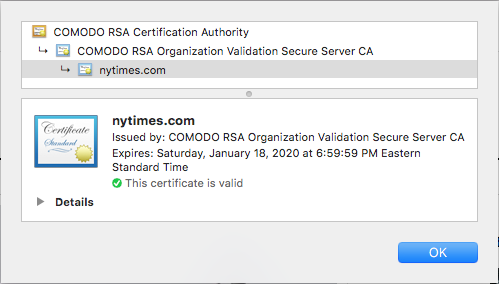
\includegraphics[width=0.7\textwidth]{ca.png}
\caption{\label{fig:ca}Example certificate chain used to authenticate the secure \nolinkurl{nytimes.com} website, as displayed in the Chrome browser.}
\end{figure}

The reality of key compromise and the wide geographical reach of large certificate authorities has led to the emergence of an alternative hierarchical PKI. This model extends the centralized approach, and still makes use of the key distribution and principal verification strategies used by the centralized model. But now, the primary ``root'' CA \emph{delegates} the ability to issue certificates to a number of subsidiary or ``second-level '' CAs. Certificates issued by second-level CAs then come with root-issued CAs themselves, thus forming a ``certificate chain'' that can be verified in sequence until reaching a trusted root CA with a known public key. 

We can formalize this delegation policy using authorization logic. All that the CA needs to do is sign propositions that denote which principals they trust to  sign on their behalf, e.g. with a predicate \trusts{\cdot}. Then the subsidiary CA can attach the policy in (\ref{eq:delegate}) signed by the root CA to any certificate that it issues using its delegation privelege.
\begin{equation}
\label{eq:delegate}
\says{\ca}{(\forall x.\forall y. \says{\ca}{\trusts{x}} \limply \says{x}{\iskey{\pk{y}}{y}} \limply \iskey{\pk{y}}{{y}})}
\end{equation}
Checking that the rules \irref{sign} and \irref{cert} described earlier allow others to make effective use of subsidiary-issued certificates is left as an exercise.

An example of this model in action is shown in Figure~\ref{fig:ca}, which is the current certificate provided when visiting \nolinkurl{https://nytimes.com}. The root CA in this case is \emph{COMODO RSA Certification Authority} (we will call this $A$), and the second-level CA is \emph{COMODO RSA Organization Validation Secure Server CA} (we will call this $B$), which is the principal who signed the public key of \nolinkurl{nytimes.com}. The browser verifies that the certificate for \nolinkurl{nytimes.com} was signed by $B$, and that the certificate for $B$ was signed by the root CA $A$. In addition, the browser will check that the root-signed certificate for $B$'s public key is authorized to sign certificates itself; this is a special ``extension'' field supported by the standard (X.509~\cite{deltacrl}) for digital certificates. This special designation essentially says that $B$ is trusted by $A$ to issue additional certificates on behalf of $A$, and that those certificates should be treated as though they were issued by $A$ itself.

The ability to delegate certification authority addresses many of the practial hurdles in the centralized CA model. Certificate authorities need to shoulder several burdens: ensuring the secrecy of the signing key, ensuring that the public key is readily available for verification, and vetting clients who wish to obtain certificates. Splitting these responsibilities among several subsidiaries makes good logistical sense. However, it also means that instead of just one signing key, there are now several that must be kept secret. The root CA must also ensure the integrity of subsidiary CAs, as they have the ability to issue certificates on behalf of the root CA, and so the trustworthiness of all related CAs is defined by the least trustworthy subsidiary. In short, while the hierarchical model solves some problems, it introduces several others.

\subsection{Web of trust}

\begin{figure}
\centering
\subfloat[]{
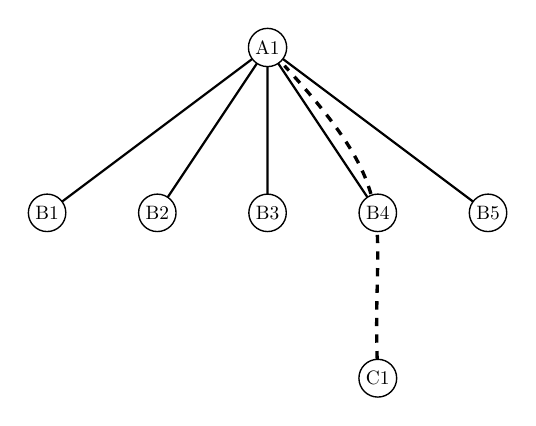
\begin{tikzpicture}[scale=0.7,transform shape]
  \Vertex[x=10,y=0]{A1}
  \Vertex[x=6,y=-3]{B1}
  \Vertex[x=8,y=-3]{B2}
  \Vertex[x=10,y=-3]{B3}
  \Vertex[x=12,y=-3]{B4}
  \Vertex[x=14,y=-3]{B5}
  \Vertex[x=12,y=-6]{C1}
  \tikzstyle{LabelStyle}=[fill=white]
  \Edge(A1)(B1)
  \Edge(A1)(B2)
  \Edge(A1)(B3)
  \Edge(A1)(B4)
  \Edge(A1)(B5)
  \path  (C1) .. controls (11.9,-3) and (12.5,-2.7) .. (A1)
     {\foreach \t [count=\i] in {0.00,0.01,...,0.99} {  coordinate[pos=\t] (p\i) } };
  \begin{pgfonlayer}{bg}
    \draw[dashed,very thick] (p1) { \foreach \i in {1,...,100} {-- (p\i) } };
  \end{pgfonlayer}
\end{tikzpicture}
}
\quad\quad\quad\quad\quad
\subfloat[]{
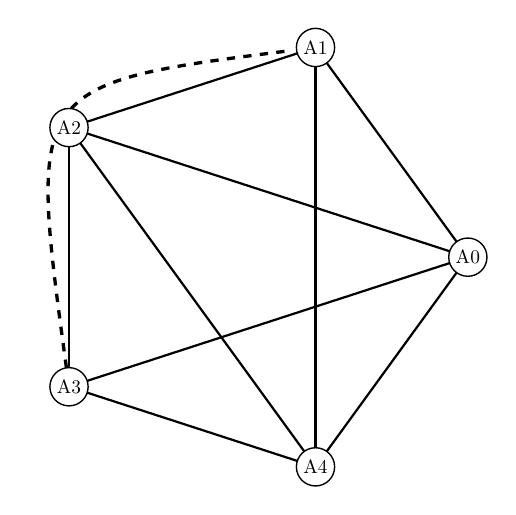
\begin{tikzpicture}[scale=0.7,transform shape]
  \grEmptyCycle[prefix=A,RA=4]{5}
  \EdgeInGraphModLoop{A}{5}{4}{1}
  \Edge(A2)(A4)
  \Edge(A2)(A0)
  \Edge(A1)(A4)
  \Edge(A0)(A3)
  \path  (A3) .. controls +(-0.75,5.5) .. (A1)
     {\foreach \t [count=\i] in {0.00,0.01,...,0.99} {  coordinate[pos=\t] (p\i) } };
  \begin{pgfonlayer}{bg}
    \draw[dashed,very thick] (p1) { \foreach \i in {1,...,100} {-- (p\i) } };
  \end{pgfonlayer}
\end{tikzpicture}
}
\caption{Hierarchical (a) and Web of Trust (b) PKI models, where solid lines correspond to existing trust relationships and dashed curves to the certificate chains that must be verified to build new ones. In the hierarchical model, A1 is the root CA, and B1-B5 are the second-level subsidiary CAs. The second-level CAs issue most certificates, so if one wants to verify C1's certificate then they need to first check that B4 signed C1's key, and then verify that A1 signed B4's key. In Web of Trust, all parties occupy a flat hierarchy, and verify certificates using previously-verified keys. If A3 wishes to authenticate A1's key, A3 can ask for a certificate  signed by A3, who is a common point of trust between the two parties. }
\end{figure}

An alternative PKI model to the hierarchical trust model is known as \emph{Web of Trust} (WOT). While the hierarchical model is widely deployed in operating systems and web browsers, WOT has been in use for several decades particularly in the context of the \emph{Pretty Good Privacy} (PGP)~\cite{Garfinkel1996} project. In WOT, trust is completely decentralized and users are responsible for making their own decisions about which certificates to trust. Likewise, every user is able to issue certificates as they wish, and distribute them at-will to others.

To get an idea of how this might work, consider a scenario where \matt wishes to send \tli an email encrypted with his secret key. He sends his public key, along with certificates $\cert{\frank}{\matt}$ signed by the department head \frank and $\cert{\jan}{\matt}$ signed by the 15-312 instructor \jan. Supposing that \tli does not know \jan, and so does not trust the latter cert, he almost certainly has received official correspondence from \frank, and has thus already established the authenticity of his public key. He can thus verify the first cert $\cert{\frank}{\matt}$, and authenticate \matt's public key prior to decrypting.

The main advantate of WOT over the prior two models is the distribution of potential failure. There are no concentrated points of failure in the event of compromise, and everyone is incentivized to proactively authenticate the public keys of anyone they communicate with. Over time, this tends to build redundancy into the system so that if any one user's signing key becomes compromised then anyone who may need to use a cert issued by them will still have several options available. 

The main drawback is scalability and usability. While WOT remains in use in the context of encrypted email, it has not become an established alternative for other applications as it is difficult and time-consuming to develop a robust network of trust relationships. Additionally, users who are not familiar with public key cryptography face hurdles in being tasked with maintaining a secure and extensive set of trust relationships and certificates, and it is not at all clear that this approach is usable outside of the relatively homogenous group of PGP devotees.

\subsection{Dealing with certificate compromise}

So far we have discussed the possible consequences of key compromise, and weighed the potential ramifications of several PKI models on this outcome. But what happens when a signing key becomes compromised? This poses a significant challenge, as continued trust in signatures issued with that key cripples the security of applications that rely on it. The CA needs to disavow, or \emph{revoke}, the compromised key immediately while ensuring that users are aware that they should no longer trust the old one. There are several approaches for doing this, none of them entirely satisfactory. At present, this remains an open and active research question.

\paragraph{Expiration.} Nearly all certificates in use today were issued with an expiration date, as shown in Figure~\ref{fig:ca}. This facilitates a ``default'' mode of protection against key compromise, as once the expiration date passes verifiers will no longer trust the certificate. However, expiration alone is not sufficient to fully address the problem, as there is an untenable conflict between scalability and the burden on CAs to continually issue and distribute new certificates, and the ``window of vulnerability'' between compromise and the certificate's expiration date. In other words, it is not considered feasible to set short certificate lifetimes of, say, one day to one week, because if this were common practice then there would be no way for CAs to keep up with the computational and bandwidth requirements needed to constantly re-issue new certificates. Typically, CA-issued certificates have lifetimes that last several years, and this leaves the parties in question with a potentially large time span in which their operations are affected by compromise.

\paragraph{Certificate revocation lists.} The most common way of handling this problem is for the CA to maintain a \emph{certificate revocation list} (CRL). Each certificate is given a unique serial number, and if the key becomes compromised then the CA is notified that the certificate with the corresponding serial number should be revoked. The CA distributes an updated CRL each day, and verifiers are responsible for cross-referencing the list when checking a certificate.

Because new CRLs must be obtained by users regularly, this solution imposes a significant burden on the PKI. Whereas before communications could take place ``offline'' without needing to communicate with services exclusive to PKI, this is no longer the case. If the CRL server goes offline, either incidentially or as the result of an explicit attack, then users can no longer verify certificates without running the risk of accepting one signed by a compromised key. Additionally, CRLs tend to grow quite large over time, and this leads to non-trivial bandwidth costs for ISPs and end-users, particularly those who operate mobile devices. While proposals for incremental CRLs exist (\cite{deltacrl}, Section 5.2.4), they are not widely implemented.

\paragraph{Online Certificate Status Protocol (OCSP).} A recent alternative to certificate revocation lists is OCSP, which is an active protocol in which parties ``pull'' information about certificate status rather than having CAs ``push'' the information routinely~\cite{ocsp}. The details of the protocol are not immediately relevant to our discussion, but it does offer some interesting tradeoffs to CRLs. The problem that OCSP alleviates is the transmission of large CRLs to end users. Because typical OCSP data transfers occur in response to specific certificate transactions, the amount of data in them is significantly smaller and therefore easier to parse and manage on resource-constrained devices. However, where connectivity or latency are issues, OCSP may become more burdensome than if an up-to-date CRL were stored on the device. 

OCSP has also raised concern from privacy advocates. The on-demand ``pull'' nature of the protocol essentially requires users to tell a central third party whose certificates they would like to validate. Because much of the web now supports HTTPS, which requires certificate validation, this means that visiting a secure website from a browser that uses OCSP (this includes Internet Explorer, Mozilla, Safari, and Opera, but not Chrome) results in the OCSP server learning that the user visited that website. To make matters worse, the OCSP proposed standard does not mandate encryption by default, so third parties sitting between the user and the OCSP server may also be able to snoop on these requests.

\paragraph{Certificate pinning.} A fairly recent practice called \emph{certificate pinning} addresses the possibility of CA key compromise. Because there are dozens of root CAs that browsers are configured to trust by default, if any one of these CAs becomes compromised then the attacker can issue certificates as that CA for \emph{any} user or domain. So suppose that \verb'cmu.edu' contracts with only one CA for certificate issuance, \tca. Now a new CA, \dca, enters the marketplace and quickly becomes compromised thanks to their lax security standards. If browsers and operating systems are already configured to trust \dca, then the party who compromised their key can now issue certificates for \verb'cmu.edu', even though \verb'cmu.edu' never used the services of \dca!

Certificate pinning addresses this by allowing parties to ``pin'' a set of trusted CAs, so that verifiers will only trust the public keys of pinned CAs chosen by \verb'cmu.edu'; in this case, \verb'cmu.edu' would only pin \tca. Certificate pinning is now common practice when configuring HTTPS websites, and is supported by all major browsers. One drawback to certificate pinning is that it can obviate legitimate network security tools that essentially use man-in-the-middle attacks to scan encrypted network traffic for malicious content. Another drawback is that if the CA becomes compromised, then nobody will be able to verify certificates pinned to that CA until the pin expiration date arrives.

\bibliography{bibliography}
\end{document}